% uklad dokumentu
	\documentclass{article}
	\usepackage{xparse}
	\usepackage[margin=1cm]{geometry}
    \usepackage{enumerate} 
	\frenchspacing
    \linespread{1.2}
    \setlength{\parindent}{0pt}

% jezyk polski
	\usepackage[polish]{babel}
	\usepackage[utf8]{inputenc}
	\usepackage{polski}
 
% pakiety matematyczne
    \let\lll\undefined
	\usepackage{amssymb}
    \usepackage{amsthm}
	\usepackage{amsmath}
	\usepackage{amsfonts}
	\usepackage{tikz}

% hiperlacza
	\usepackage{hyperref}
	\hypersetup{
		colorlinks,
		citecolor=black,
		filecolor=black,
		linkcolor=black,
		urlcolor=black
	}

% wstawianie zdjec
	\usepackage{graphicx} 
	\pagenumbering{gobble}
	

% podstawowe informacje
    \title{Algorytmy i struktury danych - Lista 4}
    \author{P. Cegieła, W. Sęk}

\begin{document} 

\maketitle
\section{Algorytm k-random}
\subsection{Tabela}
\begin{center}
\begin{tabular}{|c|c|c|c|}
\hline
\multicolumn{4}{|c|}{\textbf{Average PRD}}\\
\hline
\textbf{n} & 10-Random & 100-Random & 1000-Random\\
\hline
100 & 6413.9156401721075 & 6007.918586928952 & 5711.806977951733\\
\hline
200 & 5988.615372379403 & 5727.247304868426 & 5522.69171607988\\
\hline
300 & 5888.036831784668 & 5683.792028830031 & 5528.337270981829\\
\hline
400 & 5802.963142088209 & 5631.843379656301 & 5508.994282851\\
\hline
500 & 5779.552537965469 & 5633.505579085746 & 5517.331574583659\\
\hline
600 & 5724.137341197624 & 5578.206097637371 & 5485.583014224162\\
\hline
700 & 5711.069467439124 & 5571.201094319976 & 5476.566562989776\\
\hline
800 & 5677.560472641102 & 5562.185079759854 & 5470.719995332991\\
\hline
900 & 5673.623396583947 & 5548.007479574144 & 5481.1123195262335\\
\hline
1000 & 5650.144622314967 & 5556.232385763668 & 5459.875331845722\\
\hline
\end{tabular}
\end{center}

\subsection{Wykresy}
\begin{center}
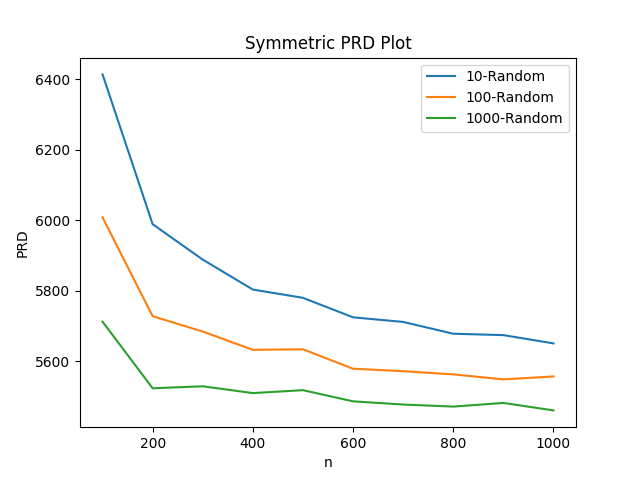
\includegraphics[width=\textwidth, 
                   height = 0.4\textheight, 
                   keepaspectratio]
                  {sym_k_random} 
\end{center}
\begin{center}
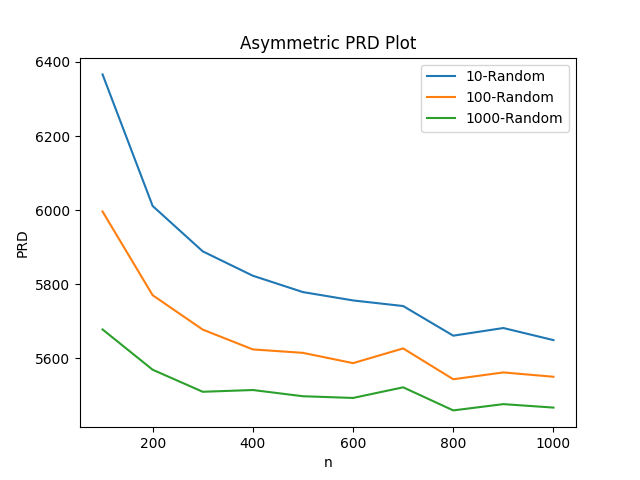
\includegraphics[width=\textwidth, 
                   height = 0.4\textheight, 
                   keepaspectratio]
                  {asym_k_random} 
\end{center}

\begin{center}
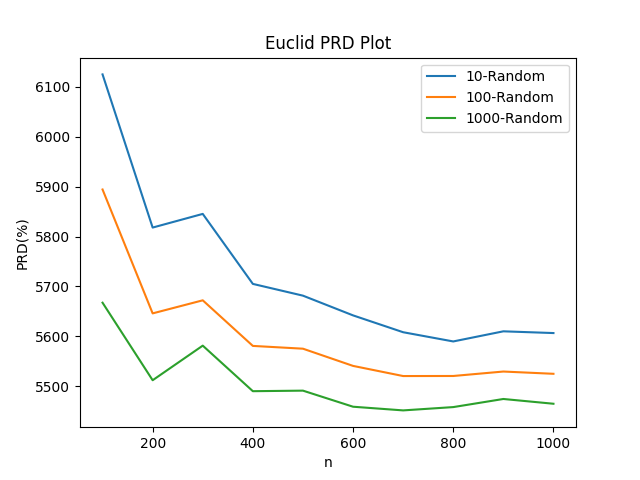
\includegraphics[width=\textwidth, 
                   height = 0.4\textheight, 
                   keepaspectratio]
                  {euc_k_random} 
\end{center}
\newpage
\section{Porównanie algorytmów na grafach euklidesowych z TSPLIB}
\subsection{Tabele}
\begin{center}
\begin{tabular}{|c|c|c|c|}
\hline
\multicolumn{4}{|c|}{\textbf{Average PRD}}\\
\hline
\textbf{n} & 1000-Random & Extended-Neighbours & 2-OPT\\
\hline
280 & 1190.481 & 105.355 & 94.110\\
\hline
52 & 313.842 & 98.473 & 92.241\\
\hline
130 & 655.514 & 105.463 & 93.669\\
\hline
150 & 722.093 & 100.510 & 91.808\\
\hline
51 & 304.930 & 103.146 & 91.878\\
\hline
76 & 390.223 & 103.011 & 92.974\\
\hline
105 & 719.383 & 107.776 & 95.285\\
\hline
442 & 1410.979 & 106.094 & 94.210\\
\hline
76 & 437.657 & 111.045 & 94.849\\
\hline
100 & 599.637 & 109.201 & 95.515\\
\hline
70 & 443.081 & 107.926 & 97.704\\
\hline
225 & 958.394 & 110.576 & 94.255\\
\hline
\end{tabular}
\end{center}

\begin{center}
\begin{tabular}{|c|c|c|c|}
\hline
\multicolumn{4}{|c|}{\textbf{Average Time}}\\
\hline
\textbf{n} & 1000-Random & Extended-Neighbours & 2-OPT\\
\hline
280 & 1824391000 & 7216115200 & 12956555100\\
\hline
52 & 337466300 & 53224900 & 100680300\\
\hline
130 & 847446300 & 776220800 & 1495083700\\
\hline
150 & 1216246900 & 1413185300 & 2831431300\\
\hline
51 & 397964700 & 70906500 & 135488700\\
\hline
76 & 529495400 & 169370500 & 342460800\\
\hline
105 & 826099200 & 562516800 & 1193324400\\
\hline
442 & 2925433800 & 28520444700 & 53773197200\\
\hline
76 & 451942500 & 153868400 & 348626900\\
\hline
100 & 599398700 & 332370900 & 876795000\\
\hline
70 & 435804700 & 123948500 & 285729600\\
\hline
225 & 1336604800 & 3619145800 & 7337685000\\
\hline
\end{tabular}
\end{center}

\begin{center}
\begin{tabular}{|c|c|c|c|}
\hline
\multicolumn{4}{|c|}{\textbf{Maximal Time}}\\
\hline
\textbf{n} & 1000-Random & Extended-Neighbours & 2-OPT\\
\hline
280 & 226062700 & 800549100 & 1374390600\\
\hline
52 & 36579000 & 5832400 & 11066200\\
\hline
130 & 103836900 & 84908600 & 173113200\\
\hline
150 & 196152300 & 201122200 & 433930400\\
\hline
51 & 52224600 & 11076500 & 18398300\\
\hline
76 & 66321000 & 20809800 & 38979800\\
\hline
105 & 103035700 & 73946000 & 164836700\\
\hline
442 & 330026000 & 3123459200 & 5680294300\\
\hline
76 & 45770600 & 15989400 & 35452500\\
\hline
100 & 61684700 & 34254200 & 90924800\\
\hline
70 & 50222300 & 15401600 & 34864000\\
\hline
225 & 137559000 & 367219200 & 757268500\\
\hline
\end{tabular}
\end{center}


\subsection{Wykresy}
\begin{center}
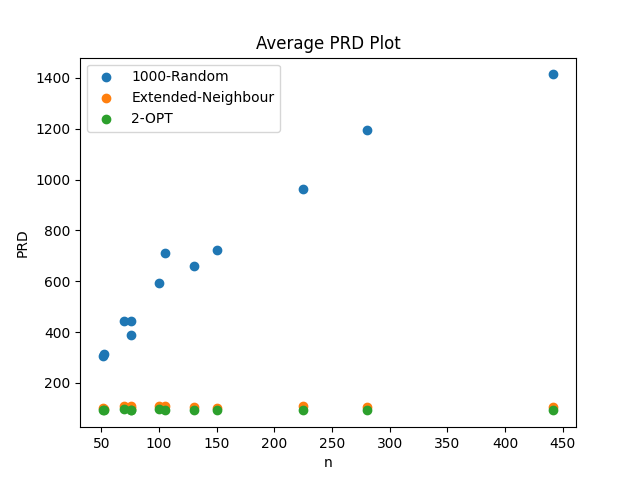
\includegraphics[width=\textwidth, 
                   height = 0.4\textheight, 
                   keepaspectratio]
                  {tsp_lib_prd} 
\end{center}
\begin{center}
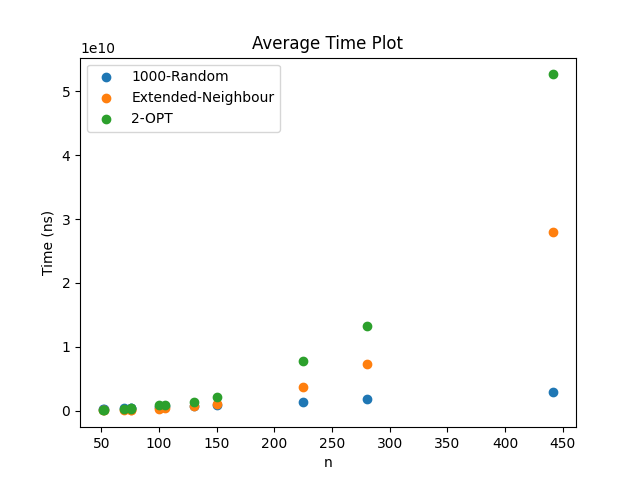
\includegraphics[width=\textwidth, 
                   height = 0.4\textheight, 
                   keepaspectratio]
                  {tsp_lib_avg_time} 
\end{center}

\begin{center}
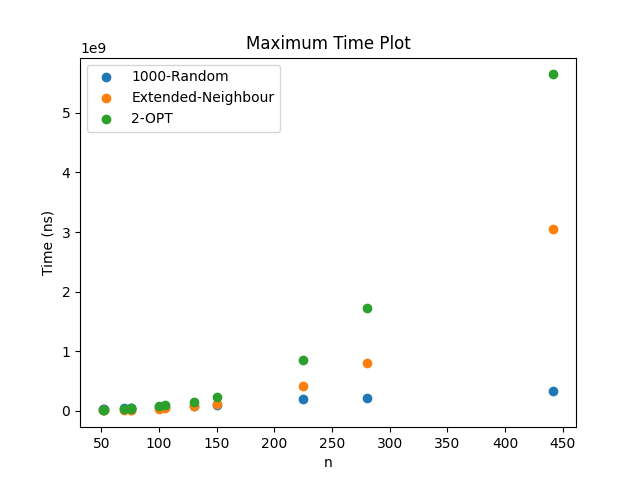
\includegraphics[width=\textwidth, 
                   height = 0.4\textheight, 
                   keepaspectratio]
                  {tsp_lib_max_time} 
\end{center}



\end{document}